%%=============================================================================
%% Inleiding
%%=============================================================================

\chapter{Inleiding}
\label{ch:inleiding}

%De inleiding moet de lezer alle nodige informatie verschaffen om het onderwerp te begrijpen zonder nog externe werken te moeten raadplegen \autocite{Pollefliet2011}. Dit is een doorlopende tekst die gebaseerd is op al wat je over het onderwerp gelezen hebt (literatuuronderzoek).

%Je verwijst bij elke bewering die je doet, vakterm die je introduceert, enz. naar je bronnen. In \LaTeX{} kan dat met het commando \texttt{$\backslash${textcite\{\}}} of \texttt{$\backslash${autocite\{\}}}. Als argument van het commando geef je de ``sleutel'' van een ``record'' in een bibliografische databank in het Bib\TeX{}-formaat (een tekstbestand). Als je expliciet naar de auteur verwijst in de zin, gebruik je \texttt{$\backslash${}textcite\{\}}.
%Soms wil je de auteur niet expliciet vernoemen, dan gebruik je \texttt{$\backslash${}autocite\{\}}. Hieronder een voorbeeld van elk.

%\textcite{Knuth1998} schreef een van de standaardwerken over sorteer- en zoekalgoritmen. Experten zijn het erover eens dat cloud computing een interessante opportuniteit vormen, zowel voor gebruikers als voor dienstverleners op vlak van informatietechnologie~\autocite{Creeger2009}.

Bedrijven kunnen tegenwoordig niet zonder IT-infrastructuur. Deze infrastructuur kan zeer uitgebreid en complex zijn. Bovendien moet het ook nog schalen naarmate het bedrijf groeit. Als systeembeheerder heb je diverse taken waaronder zaken zoals incident management en het volgen en onderzoeken van de laatste technologische trends of bedreigingen. Het opzetten en configureren van de zoveelste identieke server is dus een groot tijd- en geldverlies. Daarom werden configuration management tools in het leven geroepen. De eerst bekende tool was Puppet. Deze technologie stelde ons in staat om configuraties van servers als het ware te programmeren. Eens de gewenste configuratie geprogammeerd was konden extra gelijkaardige servers veel sneller opgezet worden. Veel systeembeheerders werden hierdoor plots DevOp genoemd. Mensen die tot nu toe enkel systeembeheer deden begonnen dus meer te programmeren, het programmeren van configuraties. 








%--------------------------------------

\section{Stand van zaken}
\label{sec:stand-van-zaken}


%% TODO: deze sectie (die je kan opsplitsen in verschillende secties) bevat je
%% literatuurstudie. Vergeet niet telkens je bronnen te vermelden!
Puppet is altijd al marktleider geweest zoals te zien is op figuur \ref{fig:popcon_everybody}. Maar daar komt nu verandering in. Er is de laatste jaren meer concurentie op de markt gekomen waaronder bekenden zoals Salt en Chef. 
Maar \'e\'en van deze nieuwe CMT 's doet het opvallend beter op gebied van populariteit en dat is Ansible inc. Zoals op de grafiek te zien is heeft Ansible in 2015 de leiding genomen. Het was ook bovendien in dat jaar dat Ansible werd vernoemd in een artikel van Gartner getiteld ?Cool Vendors in DevOps? \autocite{coolvendors}. Het was ook dat jaar dat Red Hat aankondigde dat er een akkoord was om Ansible over te nemen \autocite{redhatovername}. Voorlopig laat Ansible zijn concurenten ver achter zich.

\begin{figure}
  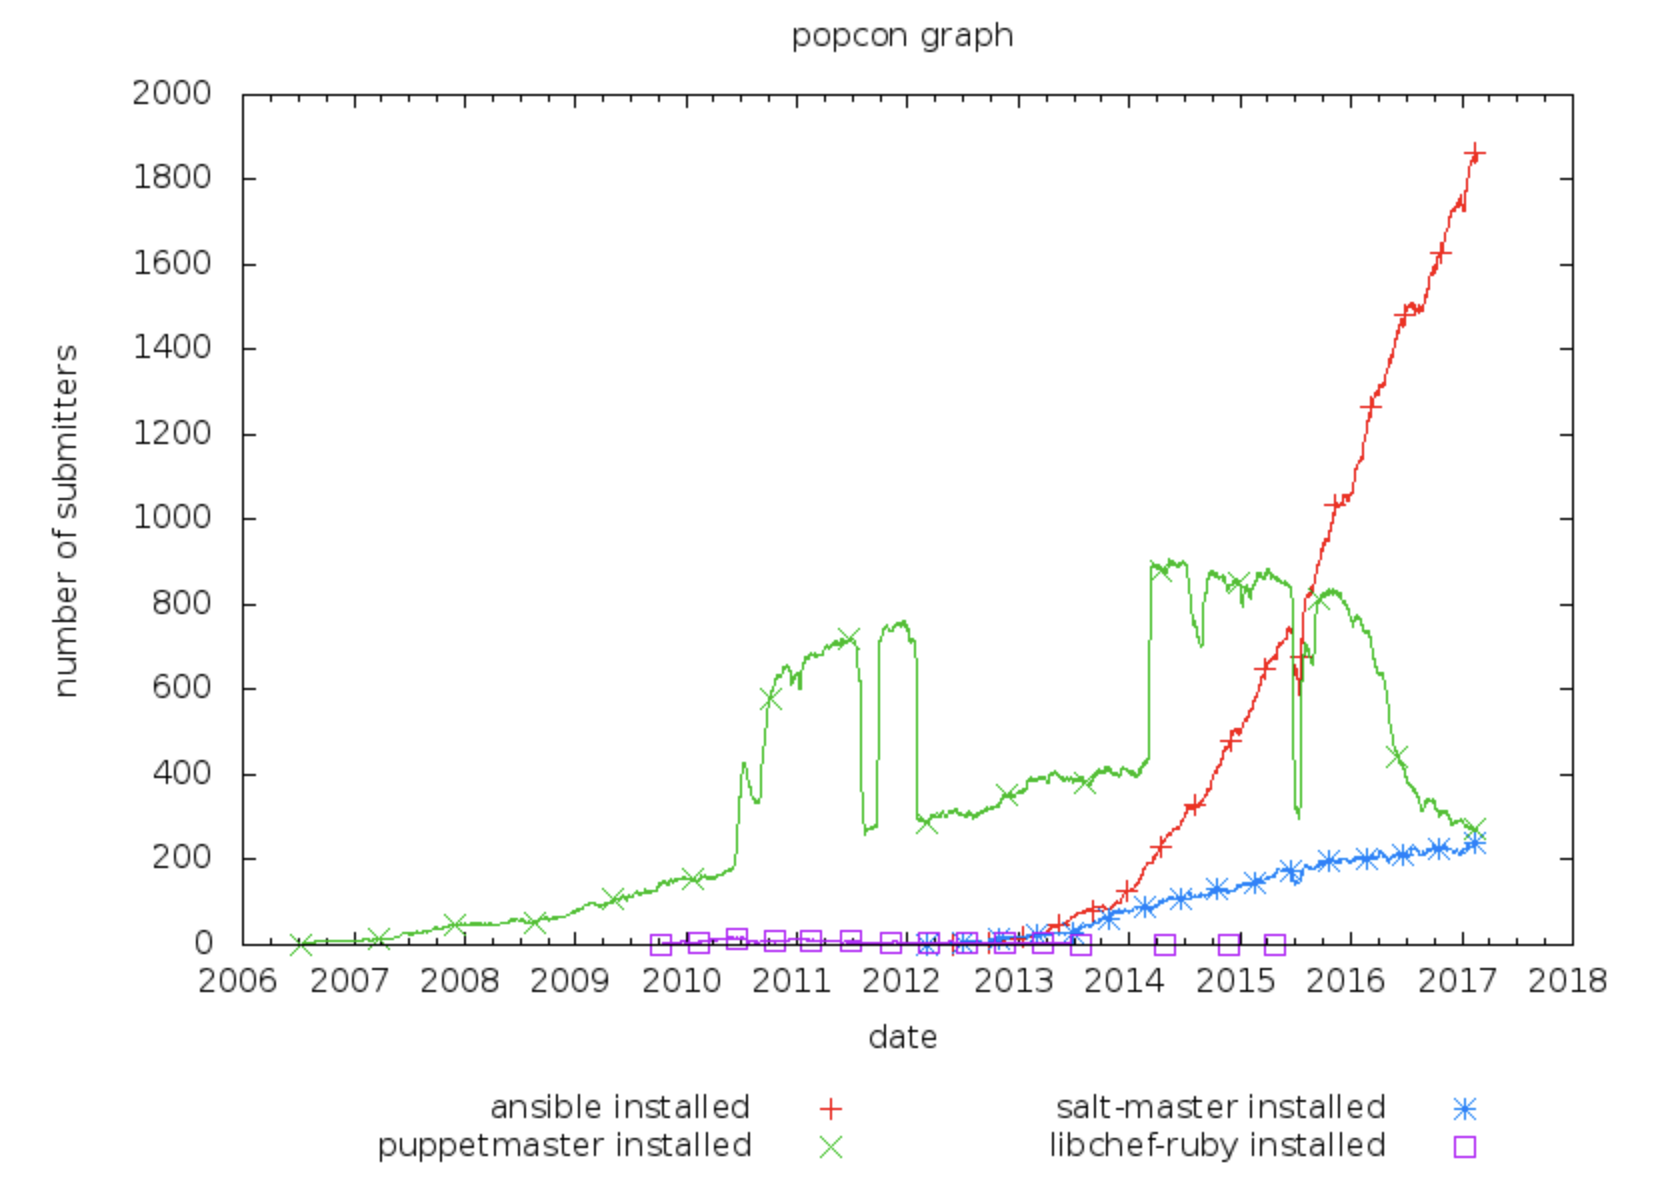
\includegraphics[width=\linewidth]{img/popcon_everybody.png}
  \caption{Deze grafiek toont het aantal keren dat een bepaald softwarepakket ge\"{\i}nstalleerd is op een debian distributie. \autocite{popcon}}
  \label{fig:popcon_everybody}
\end{figure}



\section{Opzet van deze bachelorproef}
\label{sec:opzet-bachelorproef}

In dit onderzoek vallen kleinere CMT's zoals Chef en Salt buiten de scope en zal er bijgevolg de focus gelegd worden op Puppet en Ansible. Dit onderzoek vind plaats binnen de VRT. Momenteel wordt er gebruik gemaakt van Puppet maar deze voldoet niet aan de verwachtingen van de bussiness en daarom is er dan ook besloten geweest om de huidige puppet-infrastructuur te vervangen door Ansible.
Deze bachelorproef wilt een hulp bieden aan bedrijven die dezelfde overstap overwegen. Ansible stijgt drastisch in populariteit, zoveel is zeker. Maar het is echter niet de eerste keer dat er een hype ontstond rond een onderwerp dat vervolgens gigantische teleurstelling veroorzaakte bij een community. Inmiddels heeft Ansible zich al kunnen bewijzen door possitieve analyses te krijgen van RedHat en Gartner. Maar is het zo dat Ansible het beter doet dan Puppet die inmiddels al 12 jaar ervaring heeft?




\section{Probleemstelling en Onderzoeksvragen}
\label{sec:onderzoeksvragen}

%% TODO:
%% Uit je probleemstelling moet duidelijk zijn dat je onderzoek een meerwaarde
%% heeft voor een concrete doelgroep (bv. een bedrijf).
%%
%% Wees zo concreet mogelijk bij het formuleren van je
%% onderzoeksvra(a)g(en). Een onderzoeksvraag is trouwens iets waar nog
%% niemand op dit moment een antwoord heeft (voor zover je kan nagaan).


%% TODO: Het is gebruikelijk aan het einde van de inleiding een overzicht te
%% geven van de opbouw van de rest van de tekst. Deze sectie bevat al een aanzet
%% die je kan aanvullen/aanpassen in functie van je eigen tekst.

De overschakeling van Puppet naar Ansible is geen kleine stap die ongetwijfeld voor complicaties zal zorgen. Daarom weet men best op voorhand wat er te wachten staat en wat voordelen en nadelen kunnen zijn aan deze overschakeling. Daarom zal er in dit onderzoek verschillende relevante zaken onderzocht worden. Deze kunnen opgedeeld worden in drie grote categorie\'en. 
\subsection{Wat zijn de technische voor-en nadelen van Puppet en Ansible?}

In de eerste categorie zal er een vergelijkende studie plaatsvinden waarbij technische aspecten zoals performantie, schaalbaarheid in veiligheid vergeleken worden. Onder performantie wordt verstaan de tijd die het kost tot het bekomen van een consistente staat. Dit wordt onderzocht in twee situaties, namelijk als er nog geen configuratie aanwezig is en wanneer de server reeds geconfigureerd is maar enkele aanpassingen moeten doorgevoerd worden. Een tweede aspect van deze categorie is schaalbaarheid. Onder schaalbaarheid wordt verstaan: het vermogen om grote vraag te verwerken zonder kwaliteit te verliezen \autocite{informit}. We zullen monitoren hoe Ansible en Puppet hun resources verdelen bij een toenemende drukte, hier onder de vorm van meer servers en uitgebreidere configuraties. Voor het laatste aspect van deze eerste categorie, veiligheid, zal er in de eerste plaats een literatuurstudie plaatsvinden met onderzoek naar welke veilig- heidsproblemen reeds gekend zijn en wat de best practises zijn


\subsection{Wat zijn de redenen van een omschakeling}

Dit gedeelte van het onderzoek zal zich meer op sociaal vlak afspelen. De verantwoordelijken binnen VRT voor de overstap van Puppet naar Ansible zullen een paar vragen voorgelegd krijgen, al dan niet tijdens een informeel gesprek. Op deze manier zal getracht worden de drijfveren achter hun beslissing tot overstap bloot te leggen.

\subsection{Wat is het verloop van een dergelijk transitperiode}

De omschakeling bij VRT is reeds begonnen op het moment van het schrijven van dit onderzoeksvoorstel en zal nog steeds bezig zijn tijdens het onderzoek zelf. Problemen die bij de vervanging van Puppet door Ansible optreden zullen gerap- porteerd worden en er zal onderzocht worden waarom deze optraden. Al dan niet gevonden oplossingen zullen beschreven en uitgelegd worden. Welke incidenten zich zullen voordoen, valt uiteraard moeilijk te voorspellen. Bijgevolg is de grootte van deze sectie moeilijk in te schatten.

%%In Hoofdstuk~\ref{ch:methodologie} wordt de methodologie toegelicht en worden de gebruikte onderzoekstechnieken besproken om een antwoord te kunnen formuleren op de onderzoeksvragen.

%% TODO: Vul hier aan voor je eigen hoofstukken, één of twee zinnen per hoofdstuk

%%In Hoofdstuk~\ref{ch:conclusie}, tenslotte, wordt de conclusie gegeven en een antwoord geformuleerd op de onderzoeksvragen. Daarbij wordt ook een aanzet gegeven voor toekomstig onderzoek binnen dit domein.

